\section{Comparison of available values}
The layout shown in \cref{fig:TripletLayout,fig:TripletColdmasses,tab:MagnetNamesToIDCards} 
as gathered from \cite{TodescoFidelReportPartII, TodescoB4MQXAMQXB2020}
help to get an overview which coldmasses are currently (RunII) installed in which order in the LHC.


\Cref{fig:MQXAb6Summary,fig:MQXBb6Summary} are also taken from \cite{TodescoFidelReportPartII}
and summarize the MQXA, MQXB measurements respectively. 
\textbf{The individual field measurements for the MQXA were not in the report.}


\Cref{tab:Compare,fig:Compare} list and compare all available data for $b_6$,
including the WISE error tables at collision from 2011\cite{WiseErrorTables2011} 
and 2015\cite{WiseErrorTables2015}.
Notably only every second value from the MQXA ID-cards lies withing the range of the 2015 WISE values.
The 2011 WISE values for most of the MQXB are quite different from all other sources.
The MQXB data from the FiDeL report and the ID-cards list identical values in most cases,
exception here is the Q2 left of IP1, \textbf{even though the powering of the magnets lists
different values} (the ID-cards seem to be taken from the second-highest powering measurements
but judging from the average and std-values they are very close, 
see \cref{fig:MQXBb6SummaryColdmasses}).



\newcommand{\warn}[1]{\textcolor{CernOrange}{#1}}


\begin{figure}[h!]
    \centering
    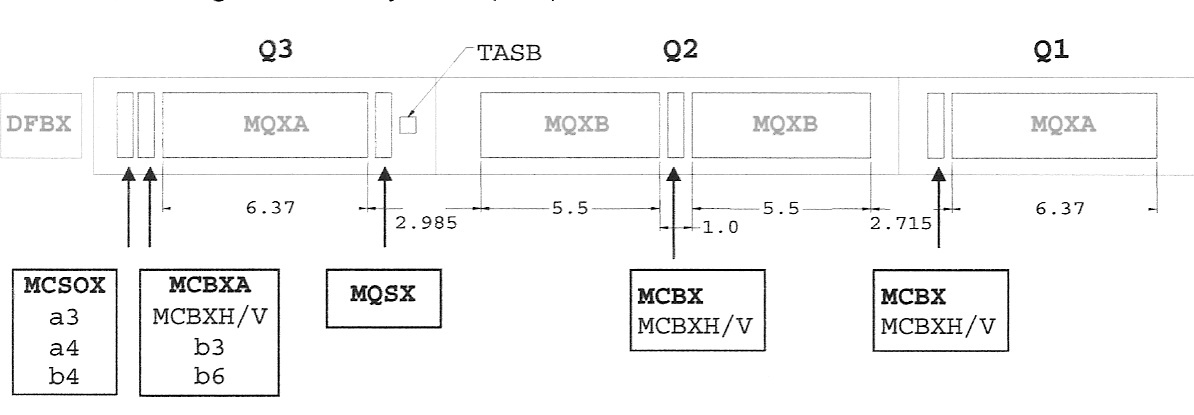
\includegraphics[width=\textwidth]{images/lhc_triplet_layout.jpg}
    \caption{Schematic LHC triplet layout}
    \label{fig:TripletLayout}
\end{figure}

\begin{figure}[h!]
    \centering
    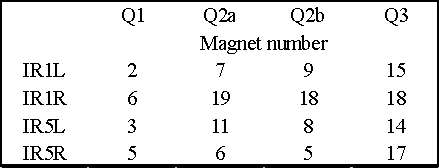
\includegraphics[width=.5\textwidth]{images/lhc_coldmass_layout.pdf}
    \caption{LHC Triplet Coldmasses}
    \label{fig:TripletColdmasses}
\end{figure}

\begin{table}[h!]
    \caption[]{ID-Card Names for installed Magnets}
    \label{tab:MagnetNamesToIDCards}
    \centering
    \begin{tabular}{lll}
        \bf Element & \bf Magnet & \bf ID-Card \\
        \toprule
        MQXA.1L1 & MQXA02 & LQXA02 \\ 
        MQXA.3L1 & MQXA15 & LQXC05 \\ 
        MQXA.1R1 & MQXA06 & LQXA06 \\ 
        MQXA.3R1 & MQXA18 & LQXC08 \\ 
        MQXA.1L5 & MQXA03 & LQXA03 \\ 
        MQXA.3L5 & MQXA14 & LQXC04 \\ 
        MQXA.1R5 & MQXA05 & LQXA05 \\ 
        MQXA.3R5 & MQXA17 & LQXC07 \\ 
        \midrule
        MQXB.A2L1 & MQXB07 & LQXB06 \\ 
        MQXB.B2L1 & MQXB09 & LQXB06 \\ 
        MQXB.A2R1 & MQXB19 & LQXB10 \\ 
        MQXB.B2R1 & MQXB18 & LQXB10 \\ 
        MQXB.A2L5 & MQXB11 & LQXB05 \\ 
        MQXB.B2L5 & MQXB08 & LQXB05 \\ 
        MQXB.A2R5 & MQXB06 & LQXB03 \\ 
        MQXB.B2R5 & MQXB05 & LQXB03 \\ 
        \bottomrule
    \end{tabular}
\end{table}


\begin{figure}[h!]
    \centering
    \begin{subfigure}{.45\textwidth}
        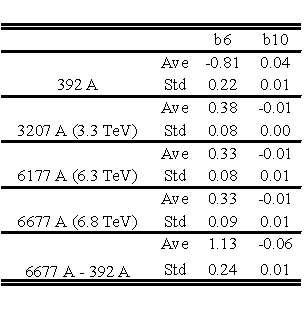
\includegraphics[width=5.11cm]{images/mqxa_b6_summary.pdf}
        \caption{Average and standard deviation over coldmasses at various fields}
    \end{subfigure}
    \begin{subfigure}{.45\textwidth}
        % \includegraphics[width=5.11cm]{images/mqxa_b6_coldmass.pdf}
        \includegraphics[width=5.11cm]{example-image}
        \caption{Individual field measurements at \SI{6677}{\ampere} (\textit{missing})}
    \end{subfigure}
    \caption{MQXA allowed multipole components}
    \label{fig:MQXAb6Summary}
\end{figure}

\begin{figure}[h!]
    \centering
    \begin{subfigure}{.45\textwidth}
        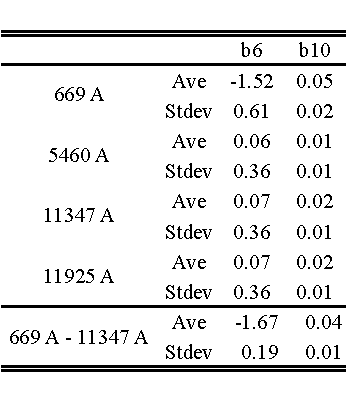
\includegraphics[width=5.11cm]{images/mqxb_b6_summary.pdf}
        \caption{Average and standard deviation over coldmasses at various field strengths}
        \label{fig:MQXBb6SummaryColdmasses}
    \end{subfigure}
    \begin{subfigure}{.45\textwidth}
        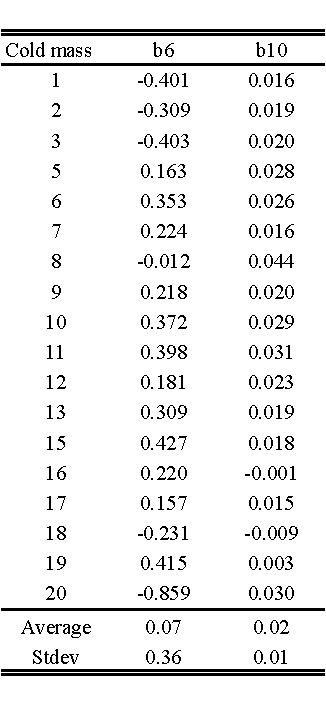
\includegraphics[width=5.11cm]{images/mqxb_b6_coldmass.pdf}
        \caption{Individual field measurements at \SI{11925}{\ampere}}
    \end{subfigure}
    \caption{MQXB allowed multipole components}
    \label{fig:MQXBb6Summary}
\end{figure}



\newcommand{\comparecap}{Comparison between $b_6$ in units from FiDeL, ID-Card and WISE 
    values at \SI{6677}{\ampere} for MQXA and 
    \SI{11925}{\ampere} (FiDeL) / \SI{11347}{\ampere} (ID-Cards) for MQXB.}
\begin{table}[h!]
    \caption[]{\comparecap}
    \label{tab:Compare}
    \small
    \centering
    \begin{tabular}{l|rrrrrrr}
        \bf Magnet &\bf FiDeL &  \bf ID-Card & \bf WISE \small{2011} & \textbf{WISE \small{2015}} Mean & Std & Min & Max \\
        \toprule
        MQXA.1L1 & - &  0.500 &  0.322 &  0.314 &  0.076 &  0.115 &  0.478 \\
        MQXA.3L1 & - &  0.251 &  0.194 &  0.195 &  0.072 & -0.013 &  0.340 \\
        MQXA.1R1 & - &  0.407 &  0.228 &  0.224 &  0.066 &  0.099 &  0.373 \\
        MQXA.3R1 & - &  0.270 &  0.213 &  0.205 &  0.080 &  0.018 &  0.365 \\
        MQXA.1L5 & - &  0.446 &  0.268 &  0.248 &  0.082 &  0.075 &  0.398 \\
        MQXA.3L5 & - &  0.301 &  0.245 &  0.248 &  0.076 &  0.067 &  0.462 \\
        MQXA.1R5 & - &  0.425 &  0.246 &  0.242 &  0.068 &  0.087 &  0.427 \\
        MQXA.3R5 & - &  0.263 &  0.206 &  0.201 &  0.085 &  0.052 &  0.373 \\
        \midrule
        MQXB.A2L1 &  \warn{0.224} &  \warn{0.218} &  0.157 &  0.167 &  0.015 &  0.131 &  0.201 \\
        MQXB.B2L1 &  \warn{0.218} &  \warn{0.210} &  0.157 &  0.160 &  0.016 &  0.126 &  0.192 \\
        MQXB.A2R1 &  0.415 &  0.415 &  0.036 &  0.359 &  0.016 &  0.327 &  0.399 \\
        MQXB.B2R1 & -0.231 & -0.231 &  0.036 & -0.288 &  0.015 & -0.320 & -0.250 \\
        MQXB.A2L5 &  0.398 &  0.398 &  0.136 &  0.344 &  0.017 &  0.308 &  0.382 \\
        MQXB.B2L5 & -0.012 & -0.012 &  0.136 & -0.069 &  0.018 & -0.111 & -0.035 \\
        MQXB.A2R5 &  0.353 &  0.353 &  0.202 &  0.293 &  0.019 &  0.256 &  0.332 \\
        MQXB.B2R5 &  0.163 &  0.163 &  0.202 &  0.104 &  0.017 &  0.062 &  0.139 \\
        \bottomrule
    \end{tabular}
\end{table}


\begin{figure}[h!]
    \centering
    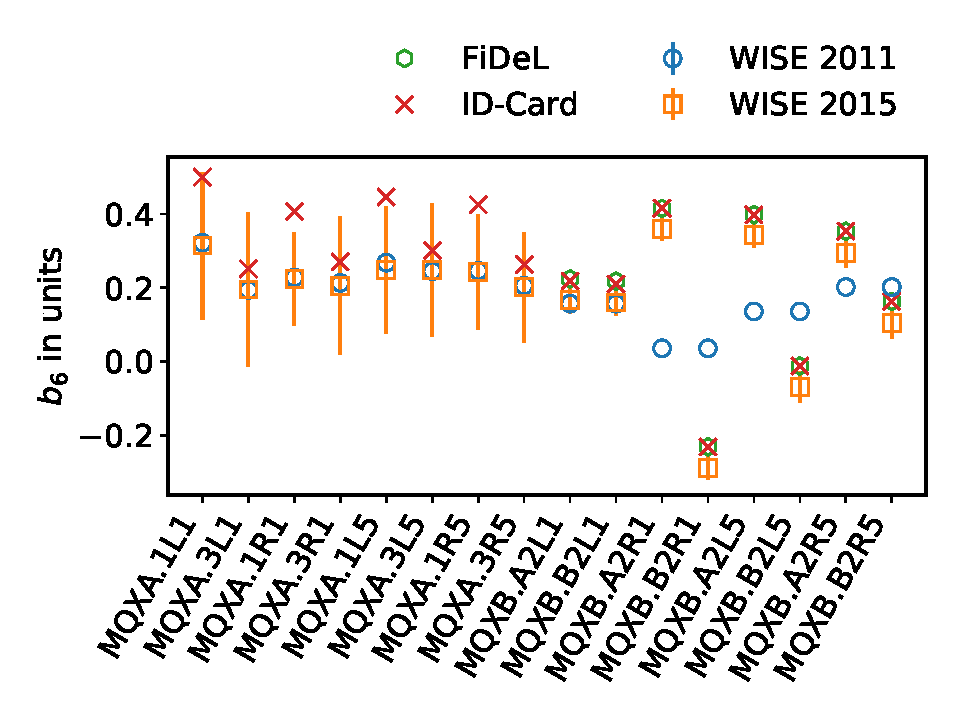
\includegraphics[width=.8\textwidth]{images/plot.Error_distributions_for_b6.pdf}
    \caption{\comparecap The errorbars indicate min and max value of the WISE 2015 data. 
    The WISE 2011 data is constant over the seeds.}
    \label{fig:Compare}
\end{figure}
